\documentclass[11pt,letterpaper]{article}
\usepackage[margin=0.92in]{geometry}
\usepackage[T1]{fontenc}
\usepackage{lmodern}
\usepackage{microtype}
\usepackage{amsmath,amssymb,amsthm,mathtools}
\usepackage{booktabs,tabularx,array}
\usepackage{enumitem}
\usepackage{xcolor}
\usepackage{hyperref}
\usepackage{tikz}
\usetikzlibrary{arrows.meta,positioning}
\hypersetup{colorlinks=true,linkcolor=blue!45!black,urlcolor=blue!45!black,pdftitle={Pure Neumann Problems in Jacobi-Simplex HPS}}
\setlist[itemize]{leftmargin=1.35em,itemsep=3pt,topsep=4pt}
\setlist[enumerate]{leftmargin=1.55em,itemsep=3pt,topsep=4pt}
\allowdisplaybreaks[1]
\newcommand{\Om}{\Omega}
\newcommand{\Gm}{\Gamma}
\newcommand{\dd}{\,\mathrm d}
\newcommand{\RR}{\mathbb R}
\newcommand{\HH}{H^1(\Om)}
\newcommand{\ip}[2]{\langle #1,#2\rangle}
\newcommand{\norm}[1]{\left\lVert#1\right\rVert}
\newcommand{\lam}{\boldsymbol\lambda}
\newcommand{\betab}{\boldsymbol\beta}
\newcommand{\qhat}{\widehat{\boldsymbol\mu}}
\newcommand{\bbroot}{\mathbf b_{\mathrm{root}}}
\newcommand{\rhs}{\mathbf h}
\newcommand{\bfone}{\mathbf 1}
\newcommand{\Ker}{\operatorname{ker}}
\newcommand{\Ran}{\operatorname{ran}}
\newcommand{\spec}{\operatorname{spec}}
\newcommand{\vol}{\operatorname{vol}}
\newcommand{\essinf}{\operatorname*{ess\,inf}}
\newcommand{\esssup}{\operatorname*{ess\,sup}}
\newtheorem{remark}{Remark}
\title{Pure Neumann Boundary Conditions\\[4pt]\large Solvability, Gauge Fixing, and Reaction Resonance\\in the Jacobi-Simplex HPS Solver}
\author{Mathematical and implementation design note - Sachin Natesh}
\date{11 October 2026}
\begin{document}
\maketitle
\vspace{-1.3em}
\begin{abstract}
We develop a single pure-Neumann treatment for the existing divergence-form
Jacobi-simplex hierarchical Poincar\'e--Steklov (HPS) discretization of
$-\nabla\cdot(A\nabla u)+b\cdot\nabla u+cu=f$.
The distinction is spectral, not a sequence of separate diffusion, advection,
and reaction implementations. For $c=0$, constants are right-null functions;
solvability requires compatibility with the \emph{adjoint} nullspace and a
user-configurable gauge selects the solution. For $c\ne0$, the constant
nullspace generally disappears, so an ordinary pure-flux boundary-value
problem may be invertible. Positive reaction gives a particularly favorable
case. Negative reaction can destroy energy coercivity without destroying
invertibility; resonance is governed by the Neumann spectrum, and general
Fredholm alternatives describe exceptional singular cases. We derive the
continuous weak and adjoint formulations, give a root-only HPS implementation
plan, and distinguish the next-release scope from more general resonant
regularization.
\end{abstract}

\section{The problem and conventions}
Let $\Om\subset\RR^D$ be a bounded, connected Lipschitz domain and set
$\Gm=\partial\Om$. Assume $A(x)$ is bounded and uniformly elliptic; unless
otherwise specified, take $A=A^T$ and
\begin{equation}
 \xi^T A(x)\xi\ge a_0|\xi|^2,\qquad a_0>0.
 \label{eq:ellipticity}
\end{equation}
The coefficients $b\in L^\infty(\Om)^D$ and $c\in L^\infty(\Om)$ are real.
Our strong problem is
\begin{equation}\label{eq:problem}
 \boxed{\begin{aligned}
 Lu:=-\nabla\cdot(A\nabla u)+b\cdot\nabla u+cu&=f
       &&\text{in }\Om,\\
 q:=n\cdot A\nabla u&=g
       &&\text{on }\Gm.
 \end{aligned}}
\end{equation}
Here $n$ is the \emph{outward} unit normal. Note that the physical diffusive
transport flux is often $J=-A\nabla u$, so $J\cdot n=-g$; that sign distinction
matters for physical conservation statements.

The weak formulation, including the inhomogeneous prescribed flux, is
\begin{equation}\label{eq:weak}
 a_c(u,v):=\int_\Om A\nabla u\cdot\nabla v\dd x
 +\int_\Om(b\cdot\nabla u)v\dd x
 +\int_\Om cuv\dd x
 =F(v),\quad v\in\HH,
\end{equation}
with
\begin{equation}\label{eq:F}
 F(v)=\int_\Om fv\dd x+\int_\Gm gv\dd S.
\end{equation}
Boundary integrals are understood via traces or normal-flux duality for the
usual Sobolev data classes. We keep the entire $A,b,c$ operator throughout.

\section{The nullspace and the exact compatibility condition}
\subsection{No reaction: $c=0$}
Since $L1=c$, for $c=0$ the constant function satisfies the homogeneous PDE
and homogeneous co-normal condition. On a connected domain, under the standard
uniform-ellipticity and regularity hypotheses, the homogeneous Neumann
problem has a one-dimensional right nullspace spanned by $1$ (including with
bounded first-order drift). Consequently, if a solution exists then $u+C$ is
also a solution.

For $b=0$, take $v=1$ in \eqref{eq:weak}. The diffusion term vanishes and we
obtain the \emph{physical conservation constraint}
\begin{equation}\label{eq:balance}
 \boxed{\int_\Om f\dd x+\int_\Gm g\dd S=0.}
\end{equation}
This is necessary and, for the connected uniformly elliptic diffusion problem,
sufficient for solvability modulo constants. It constrains only the total flux;
it does not determine the spatial function $g$ from $f$.

For nonzero drift, testing \eqref{eq:weak} with $1$ instead gives
$\int_\Om b\cdot\nabla u=F(1)$, so \eqref{eq:balance} is no longer the
correct data-only compatibility condition in general.

\subsection{Adjoint compatibility for $b\ne0$}
The formal interior adjoint and its homogeneous boundary condition are
\begin{equation}\label{eq:adjoint}
 \begin{aligned}
 L^*\phi&=-\nabla\cdot(A^T\nabla\phi)
               -\nabla\cdot(b\phi)+c\phi=0
               &&\text{in }\Om,\\
 n\cdot A^T\nabla\phi+(b\cdot n)\phi&=0
               &&\text{on }\Gm.
 \end{aligned}
\end{equation}
Integration by parts, using the primal flux $n\cdot A\nabla u=g$, yields
\begin{align}\label{eq:green}
 \int_\Om\phi Lu\dd x
 &=\int_\Om uL^*\phi\dd x
   +\int_\Gm u\bigl[n\cdot A^T\nabla\phi
                         +(b\cdot n)\phi\bigr]\dd S
   -\int_\Gm\phi g\dd S.
\end{align}
Thus every homogeneous adjoint null function imposes
\begin{equation}\label{eq:adjcompat}
 \boxed{F(\phi)=\int_\Om\phi f\dd x
                 +\int_\Gm\phi g\dd S=0,
       \qquad \phi\in\Ker L^*.}
\end{equation}
For $b=c=0$, $\phi=1$ is the adjoint null function and this reduces to
\eqref{eq:balance}. For general $b\ne0$, $\phi$ is usually nonconstant.
\emph{The implementation need not solve a second continuous adjoint PDE:}
the discrete HPS root operator already has a left nullspace that captures its
algebraic compatibility condition.

\subsection{Gauge: a uniqueness condition, not a compatibility correction}
For compatible data and $c=0$, fix a linear functional $\mathcal G$ satisfying
$\mathcal G(1)\ne0$ and prescribe
\begin{equation}\label{eq:gauge}
 \boxed{\mathcal G(u)=\eta,\qquad \eta\in\RR.}
\end{equation}
A convenient root-only choice is the physical boundary mean,
\begin{equation}\label{eq:boundarymean}
 \mathcal G_\partial(u)=\frac{1}{|\Gm|}
       \int_\Gm u\dd S.
\end{equation}
It differs from a zero-\emph{volume}-mean gauge but fixes the same additive
constant. Allow $\eta=0$ by default and expose $\eta$ to the caller.
For example, if $u_*$ is a manufactured solution, the boundary-mean-gauged
reference is $u_*+\eta-\mathcal G_\partial(u_*)$.
The solver should \emph{reject} incompatible input, rather than silently
projecting or modifying $f$ or $g$.

\section{Why prescribed Neumann data can be solvable when $c\ne0$}
The phrase \emph{pure Neumann} specifies the boundary data, not the presence
of a nullspace. Indeed $L1=c$, so a nonzero reaction term generally removes
constants from the kernel. The boundary-value operator may be invertible
without any special gauge or compatibility test. Invertibility is a property
of the \emph{entire operator} (coefficients, domain, and boundary condition),
not a consequence of the word ``Neumann.''

\subsection{Positive reaction: the Lax--Milgram case}
Suppose first $b=0$, $A=A^T$ satisfies \eqref{eq:ellipticity}, and
\begin{equation}\label{eq:cpositive}
 c(x)\ge c_0>0\quad\text{a.e. in }\Om.
\end{equation}
Then
\begin{equation}\label{eq:coercive}
 a_c(u,u)\ge a_0\norm{\nabla u}_{L^2}^2
                     +c_0\norm{u}_{L^2}^2
           \ge C\norm{u}_{H^1}^2,
 \qquad C=\min(a_0,c_0)>0.
\end{equation}
The form is bounded and coercive on all of $H^1(\Om)$; Lax--Milgram gives a
unique weak solution for each continuous functional $F$, with \emph{no}
compatibility condition and \emph{no} gauge. If $c\ge0$ is not identically
zero, diffusion plus a reaction region of positive measure also removes the
constant kernel; a generalized Poincar\'e inequality yields coercivity under
standard hypotheses, even if $\essinf c=0$.

With advection $b\ne0$, the bilinear form is nonsymmetric. A direct sufficient
Lax--Milgram condition follows from Young's inequality:
\begin{align}\label{eq:driftbound}
 \left|\int_\Om(b\cdot\nabla u)u\dd x\right|
 &\le\norm b_{L^\infty}\norm{\nabla u}_{L^2}\norm u_{L^2}\\
 &\le\frac{a_0}{2}\norm{\nabla u}_{L^2}^2
      +\frac{\norm b_{L^\infty}^2}{2a_0}\norm u_{L^2}^2,
\end{align}
so coercivity is immediate if
\begin{equation}\label{eq:driftcondition}
 c_0>\frac{\norm b_{L^\infty}^2}{2a_0}.
\end{equation}
\textbf{This is sufficient, not necessary.} For regular, uniformly elliptic
scalar operators with $c\ge c_0>0$, the maximum principle and the Neumann
boundary point principle provide uniqueness even when
\eqref{eq:driftcondition} fails; Fredholm existence then gives well-posedness.
Thus positive reaction is not intrinsically troublesome for the general
$A,b,c$ solver.

\section{Negative reaction and the Neumann spectral threshold}
\subsection{The correct indexing of Neumann eigenvalues}
Here the natural spectral analysis begins with $b=0$ and symmetric $A$.
Let $L_0=-\nabla\cdot(A\nabla)$ with homogeneous co-normal Neumann data.
The operator is self-adjoint and nonnegative on $L^2(\Om)$ with compact
resolvent. Its eigenvalues are
\begin{equation}\label{eq:spectrum}
 \boxed{0=\lambda_0^N<\lambda_1^N\le\lambda_2^N\le\cdots,
 \qquad\lambda_k^N\to\infty.}
\end{equation}
The \emph{smallest} Neumann eigenvalue is zero. The threshold commonly
intended in a negative-reaction comparison is therefore the \emph{first
positive} eigenvalue $\lambda_1^N$, not $\lambda_0^N$.
The associated weighted Poincar\'e--Rayleigh characterization is
\begin{equation}\label{eq:rayleigh}
 \lambda_1^N
 =\inf_{\substack{v\in H^1(\Om),\,v\ne0\\\int_\Om v\dd x=0}}
 \frac{\int_\Om \nabla v\cdot A\nabla v\dd x}
      {\int_\Om v^2\dd x}>0.
\end{equation}

\subsection{Constant negative reaction $c=-\mu$}
Put $\mu>0$ and set $L_\mu=L_0-\mu I$. Its spectrum is
\begin{equation}\label{eq:shiftedspec}
 \spec(L_\mu)=\{\lambda_k^N-\mu:k\ge0\}.
\end{equation}
Hence
\begin{equation}\label{eq:resonancecriterion}
 \boxed{L_\mu\text{ is invertible precisely when }
              \mu\notin\{\lambda_k^N:k\ge0\}.}
\end{equation}
In particular, every $0<\mu<\lambda_1^N$ gives a unique solution for any
admissible $f,g$, even though the full energy
$a_{-\mu}(1,1)=-\mu|\Om|$ is negative and Lax--Milgram \emph{coercivity on
all of $H^1$ fails}.

To see the useful remaining coercivity, decompose
$u=m+v$ with $m=|\Om|^{-1}\int_\Om u$ and $\int_\Om v=0$.
Equation \eqref{eq:weak} tested with $1$ gives
\begin{equation}\label{eq:meanfixed}
 -\mu|\Om|m=F(1),\qquad
 m=-\frac{F(1)}{\mu|\Om|}.
\end{equation}
The mean-zero component solves
\begin{equation}\label{eq:meansubspace}
 \int_\Om A\nabla v\cdot\nabla\psi\dd x
 -\mu\int_\Om v\psi\dd x=F(\psi)
 \quad\forall\psi\in H^1(\Om),\ \int_\Om\psi\dd x=0,
\end{equation}
and Rayleigh--Poincar\'e implies
\begin{equation}\label{eq:restrictedcoercivity}
 \int_\Om \nabla v\cdot A\nabla v\dd x-\mu\int_\Om v^2\dd x
 \ge\left(1-\frac\mu{\lambda_1^N}\right)
       \int_\Om\nabla v\cdot A\nabla v\dd x.
\end{equation}
Therefore Lax--Milgram applies on the mean-zero subspace when
$\mu<\lambda_1^N$; the constant coefficient $m$ is determined by
\eqref{eq:meanfixed}, not chosen by a gauge.

\begin{center}
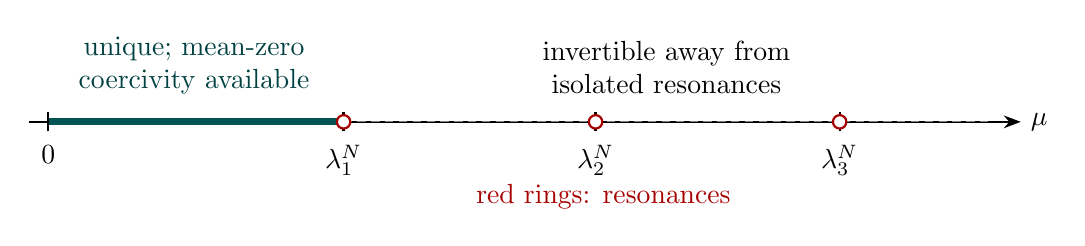
\begin{tikzpicture}[>=Stealth,scale=1]
 \draw[->,line width=.7pt] (0,0)--(12.6,0) node[right] {$\mu$};
 \draw[line width=2.5pt,teal!65!black] (.23,0)--(4.0,0);
 \draw[densely dashed,gray] (4,0)--(12.2,0);
 \foreach \x/\lab in {0.25/{0},4/{\lambda_1^N},7.2/{\lambda_2^N},10.3/{\lambda_3^N}} {
   \draw[thick] (\x,-.12)--(\x,.13);
   \node[below=5pt] at (\x,0) {$\lab$};
 }
 \foreach \x in {4,7.2,10.3} {\fill[white] (\x,0) circle (.085);\draw[red!65!black,thick] (\x,0) circle (.085);}
 \node[above,align=center,text=teal!50!black] at (2.1,.23) {unique; mean-zero\\coercivity available};
 \node[above,align=center] at (8.1,.23) {invertible away from\\isolated resonances};
 \node[below=19pt,text=red!65!black] at (7.3,0) {red rings: resonances};
\end{tikzpicture}
\end{center}

\paragraph{Above the threshold.}
For $\mu>\lambda_1^N$, the operator is \emph{not automatically singular}.
It is invertible between successive Neumann eigenvalues, but the energy has
additional negative directions. At $\mu=\lambda_k^N$, a nonconstant
homogeneous nullspace appears; solvability requires orthogonality of the
forcing functional $F$ to the corresponding eigenfunctions. A constant-only
gauge does not handle these resonances. Near them, the inverse norm can
become large, approximately like the reciprocal distance to the spectrum.

\paragraph{One-dimensional example.}
On $(0,1)$ with $A=1$,
$\lambda_k^N=k^2\pi^2$ and the normalized eigenfunctions are constants and
$\cos(k\pi x)$, $k\ge1$. For
$-u''-\mu u=f$ with $u'(0)=u'(1)=0$ (in the outward-flux convention), every
$0<\mu<\pi^2$ is uniquely solvable. At $\mu=\pi^2$, the forcing must satisfy
$\int_0^1 f(x)\cos(\pi x)\dd x=0$; when compatible, a separate condition
must fix the coefficient of $\cos(\pi x)$.

\subsection{Variable negative reaction}
For $c(x)=-\mu\rho(x)$ with $\rho\ge\rho_0>0$, the appropriate thresholds
are generalized eigenvalues of
\begin{equation}\label{eq:generalizedeigen}
 \int_\Om A\nabla\psi\cdot\nabla v\dd x
 =\nu\int_\Om\rho\psi v\dd x,
 \qquad v\in\HH.
\end{equation}
The first positive generalized eigenvalue is obtained by restricting to
$\rho$-weighted mean-zero functions and minimizing the corresponding
Rayleigh quotient. As above, $0<\mu<\nu_1$ gives an invertible operator,
while singularity occurs at generalized eigenvalues. For a completely general
sign-changing $c(x)$, a pointwise comparison of $c(x)$ with a single number
$\lambda_1^N$ is \emph{not} a complete solvability criterion: one must analyze
the full potential-perturbed operator.

\subsection{What changes when $b\ne0$?}
The diffusion--advection operator
$L_0=-\nabla\cdot(A\nabla)+b\cdot\nabla$ with Neumann flux still satisfies
$L_0 1=0$; however it is generally \emph{nonsymmetric}. Its spectrum and
adjoint eigenspaces need not admit a real Rayleigh-quotient ordering, and
spectral values may be complex. A constant reaction shift $-\mu I$ still
moves the spectrum, but the self-adjoint threshold $\lambda_1^N$ is not
available without additional symmetrizing structure. At singular values one
must use the left and right kernels of the actual operator.

\section{Fredholm alternative and regularization at resonance}
For bounded $\Om$, uniformly elliptic $A$, and bounded lower-order
coefficients, one can choose a sufficiently large $\gamma>0$ such that
$a_c(u,v)+\gamma(u,v)_{L^2}$ is coercive (by Young's inequality).
The shifted solution map is bounded, and the compact embedding
$H^1(\Om)\hookrightarrow L^2(\Om)$ yields a compact-resolvent/Fredholm
formulation for the corresponding homogeneous-boundary operator.
The Fredholm alternative states that either the operator is invertible, or
its kernel is finite dimensional and the data must annihilate every adjoint
null function. More explicitly, if
\begin{equation}\label{eq:fredholm}
 \Ker L^*=\operatorname{span}\{\phi_1,\ldots,\phi_r\},
\end{equation}
with adjoint boundary conditions \eqref{eq:adjoint}, then solvability requires
\begin{equation}\label{eq:fredholmcompat}
 \boxed{F(\phi_j)=0,\qquad j=1,\ldots,r.}
\end{equation}
When it holds, solutions differ by elements of $\Ker L$, and $r$
independent gauge functionals may be needed. This applies to negative and
sign-changing reaction terms and, with the appropriate adjoint, to drift.

\paragraph{No regularization when already invertible.}
If a negative-reaction operator is away from resonance, solve the original
problem directly. Lack of coercivity does not imply a need for Tikhonov
regularization or limiting absorption.

\paragraph{Complex resolvent shift / limiting absorption.}
For a self-adjoint real operator $L$ having a zero eigenvalue, one may
consider $(L+i\varepsilon I)u_\varepsilon=F$ with
$\varepsilon\downarrow0$. For forcing orthogonal to $\Ker L$,
$u_\varepsilon$ converges to the solution in $(\Ker L)^\perp$; otherwise
the component along the nullspace grows like $1/\varepsilon$.
On a bounded domain with discrete spectrum this is most accurately viewed
as a \emph{resolvent regularization}, not as a necessary physical radiation
condition. The non-self-adjoint case requires additional care (including
possible nonnormality and generalized eigenspaces).

\paragraph{Tikhonov regularization.}
At the discrete level one can minimize
\begin{equation}\label{eq:tikh}
 \norm{R\lam-\rhs}_2^2
 +\varepsilon^2\norm{C(\lam-\lam_{\mathrm{ref}})}_2^2,
 \qquad\varepsilon>0.
\end{equation}
As $\varepsilon\to0$, compatible data give a selected solution according
to the regularization metric and reference vector; incompatible data instead
give a least-squares compromise, \emph{not} a solution to the original PDE.
We should therefore retain an explicit compatibility test before any such
regularized solve. The gauge selected by Tikhonov is not automatically the
user's desired physical mean gauge.

\section{Root-only integration with the existing HPS solver}
\subsection{What is already available}
The Dense divergence-form HPS solver represents an exterior trace vector
$\lam\in\RR^{N_B}$ in a common canonical face Jacobi basis and supplies an
affine numerical co-normal flux map
\begin{equation}\label{eq:dtn}
 \qhat=S_{\mathrm{root}}\lam+\bbroot.
\end{equation}
The map $S_{\mathrm{root}}$ comes from the existing tau-stabilized leaf
and merge algebra; $\bbroot$ is updated from the interior source.
Pure Neumann with $\alpha=0$, $\beta=1$ therefore gives
\begin{equation}\label{eq:root}
 \boxed{R\lam=\rhs,\qquad
 R=S_{\mathrm{root}},\qquad \rhs=\mathbf g-\bbroot.}
\end{equation}
When $\beta=1$ is constant, the higher-degree co-normal flux correction
$M_\beta^{LH}$ is zero by orthogonality, so no additional high-mode term
is required. The co-normal operator already incorporates variable $A$ and
interface flux continuity.

For $\alpha=0$ but spatially varying, nowhere-vanishing $\beta$, the
already-implemented corrected variable-Robin equation instead uses
\begin{equation}\label{eq:variablebeta}
 R=M_\beta^{LL}S_{\mathrm{root}}+M_\beta^{LH}H_{\mathrm{root}},\qquad
 \rhs=\mathbf g-M_\beta^{LL}\bbroot-M_\beta^{LH}z_{\mathrm{root}}.
\end{equation}
The same nullspace methodology applies. If $\beta$ vanishes, the boundary
operator may change type and requires a separate well-posedness analysis.

\subsection{Singular constant-nullspace case, usually $c=0$}
Let $v\in\RR^{N_B}$ be the coefficient vector of the \emph{constant exterior
trace}. For an exact singular pure-Neumann root map, $Rv=0$.
Numerically $Rv$ will only be small, so assess its residual against the
operator scale and verify the expected rank deficiency rather than declaring
all ill-conditioned operators to have a constant nullspace.
Find a left-null
vector $\ell$ (e.g. using an SVD or a suitably rank-revealing factorization):
\begin{equation}\label{eq:discretekernels}
 Rv\simeq0,\qquad R^T\ell\simeq0,\qquad
 \ell^T\ell=1.
\end{equation}
The discrete compatibility condition is
\begin{equation}\label{eq:discretecompat}
 \boxed{\ell^T\rhs\simeq0.}
\end{equation}
Use a scaled, conditioning-aware tolerance, report the normalized defect,
and reject inconsistent data. The left vector $\ell$ need not coincide with
the constant trace or with a coefficient-wise vector of ones, especially
in nonsymmetric, weighted coordinates.

Construct a root boundary-mean row $w^T$ using physical face integration
and normalize it such that $w^Tv=1$. The caller supplies $\eta$ and the
gauge is $w^T\lam=\eta$. A convenient bordered root system is
\begin{equation}\label{eq:bordered}
 \boxed{
 \begin{bmatrix}R&\ell\\w^T&0\end{bmatrix}
 \begin{bmatrix}\lam\\\sigma\end{bmatrix}
 =\begin{bmatrix}\rhs\\\eta\end{bmatrix}.}
\end{equation}
If $R$ has precisely a one-dimensional right and left nullspace and
$w^Tv\ne0$, this system is nonsingular. For compatible data, $\sigma$ is
zero to numerical tolerance; $\sigma$ must not be used silently to absorb
an incompatible RHS. The gauge affects only the constant component and does
not alter the physical gradient/flux. No changes to leaf solves, interface
merges, or high co-normal observations are needed.

\subsection{What happens for $c\ne0$?}
For an ordinary well-posed pure-Neumann problem with reaction, use the
existing nonsingular root solve, including the current LU factorization.
\emph{Do not impose a constant gauge merely because $\alpha=0$.}
If the root matrix is singular or nearly singular at a reaction resonance,
report the condition/rank diagnostic. Its null modes may be nonconstant;
proper treatment would require a generalized left/right-nullspace procedure
and is outside the near-term singular-Neumann implementation.

\subsection{Proposed solver contract}
\begin{enumerate}
 \item Assemble the ordinary Dense divergence-form HPS tree and root flux map.
 \item Accept $\alpha=0$, $\beta=1$ on all exterior faces as a legitimate
       \emph{boundary specification}, regardless of $b$ and $c$.
 \item For a verified constant-nullspace case ($c=0$ within a deliberate
       coefficient-identification rule), construct the right constant trace,
       compute/validate the root left nullspace, and check
       \eqref{eq:discretecompat}.
 \item If compatible, apply the boundary-mean gauge
       $w^T\lam=\eta$ using \eqref{eq:bordered}; default $\eta=0$.
 \item If the root operator is nonsingular (notably when $c>0$ and the
       problem is well posed), use the normal solve and no gauge.
 \item If an unanticipated nonconstant nullspace/resonance is detected,
       report it rather than assigning a spurious constant gauge.
\end{enumerate}
A special explicit \texttt{pure\_neumann} flag could guard the singular branch;
for general $\alpha,\beta$ the existing Robin code remains authoritative.
The degree-$n$ HPS skeleton, tau parameter, and Dense-only divergence-form
restriction remain unchanged.

\section{Validation plan and release boundary}
The first implementation can exercise the \emph{general} $A,b,c$ operator
without staging different PDE solvers. Suggested tests on the already used
conforming simplex decompositions of the unit cube are summarized below.

\begin{center}
\small
\begin{tabularx}{\textwidth}{@{}p{.16\textwidth}p{.34\textwidth}X@{}}
\toprule
Test & Coefficients and data & Required outcome\\
\midrule
A & $A$ cubic SPD, $b=c=0$; degree-5 polynomial $u_*$, exact $f,g$ & Compatibility accepted; $u_*+C$ recovered to numerical precision under prescribed boundary-mean gauge.\\
B & Same $A$; nonzero polynomial $b$, $c=0$ & Generalized \emph{left-null} compatibility accepted; exact polynomial recovery under the gauge.\\
C & As B with $c(x)\ge c_0>0$ & Nonsingular ordinary root solve with no gauge.\\
D & Perturb only $g$ by a nonzero constant in A or B & Compatibility rejected with a diagnostic (no silent projection).\\
E & Repeat A or B with two gauge right-hand sides $\eta_1,\eta_2$ & Solutions differ by the constant $\eta_2-\eta_1$ when $w^Tv=1$; gradients and fluxes unchanged.\\
F (later) & $b=0$, constant $c=-\mu$ near/at $\lambda_k^N$ & Invertible away from resonance; reject or separately regularize resonant cases.\\
\bottomrule
\end{tabularx}
\end{center}

The current mixed Neumann/Dirichlet/variable-Robin manufactured-solution
regressions already recover the degree-5 global polynomial to roundoff in
$D=1,2,3$ and require \emph{no} nullspace machinery. The specific addition
here is the \emph{all-Neumann} singular branch, together with a nonsingular
reaction case and informative treatment of exceptional resonances.

\section{Conclusions}
\begin{enumerate}
 \item Pure Neumann means prescribed co-normal flux on every exterior face.
       It does \emph{not} inherently mean that the operator is singular.
 \item If $c=0$, constants are right-null modes. For general drift $b$, test
       compatibility against the \emph{left/adjoint} nullspace, then impose
       a caller-configurable gauge, preferably the boundary mean at the root.
 \item A strictly positive reaction makes the diffusion problem coercive;
       with drift, maximum-principle and Fredholm arguments cover cases
       beyond the simple sufficient Lax--Milgram estimate.
 \item For negative constant reaction $c=-\mu$ in the self-adjoint case,
       the first positive Neumann eigenvalue $\lambda_1^N$ marks the loss of
       coercivity on mean-zero functions. Invertibility fails only at the
       discrete resonances $\mu=\lambda_k^N$; there is no blanket
       ill-posedness for $\mu>\lambda_1^N$.
 \item Fredholm compatibility, resonant mode gauges, complex shifts, and
       Tikhonov methods provide a principled route to broader indefinite
       problems, but need not block the next release's nonresonant Neumann
       implementation.
\end{enumerate}
\end{document}
